\subsubsection{UC20 - Aggiornamento codice funzione}
\begin{figure}[h]
	\centering
	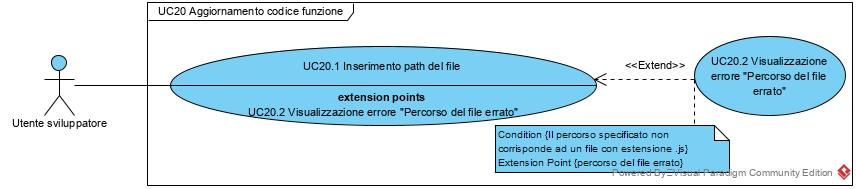
\includegraphics[width=\linewidth]{res/img/UC20.jpg}
	\caption{Diagramma UC20 - Aggiornamento codice funzione}
\end{figure}
\begin{itemize}
	\item \textbf{Attori primari:} Utente sviluppatore;
	\item \textbf{Descrizione:} l'utente potrà eseguire nuovamente il \textit{"deploy\glos"} di una sua funzione preesistente, aggiornandone il codice;
	\item \textbf{Pre-condizioni:} l'utente possiede una funzione JavaScript sul proprio dispositivo;
	\item \textbf{Post-condizioni:} il sistema si occuperà di aggiornare il codice della funzione da lui già condivisa su \textit{Etherless}. L'utente visualizzerà a schermo l'esito del comando;
	\item \textbf{Scenario principale:}
	\begin{enumerate}
		\item L'utente tramite il comando "update" aggiorna il codice di una sua funzione;
		\item Il sistema visualizzerà su schermo l'esito dell'operazione.
	\end{enumerate}
	\item\textbf{Estensioni:}
	\begin{itemize}
		\item \textbf{UC21}: il nome della funzione non è tra quelle caricate dall'utente.
	\end{itemize}
\end{itemize}
